\section{MODELO Y APLICACIÓN}
\subsection{¿Por qué PacMan?}
\begin{frame}{MODELO Y APLICACIÓN}
    \framesubtitle{¿Por qué PacMan?}
    \begin{itemize}
      \item Es considerado uno de los juegos más influyentes en la cultura mundial. Fue desarrollado por Toru Iwanati en 1979\footnote{\bibentry{pac}}.
      \item Los videojuegos estaban en su etapa temprana y los desarrolladores carecían de algoritmos para mejorar la experiencia en juego.
      \item Los enemigos no presentan mayor problema para completar el juego.
    \end{itemize}
    \begin{figure}[H]
      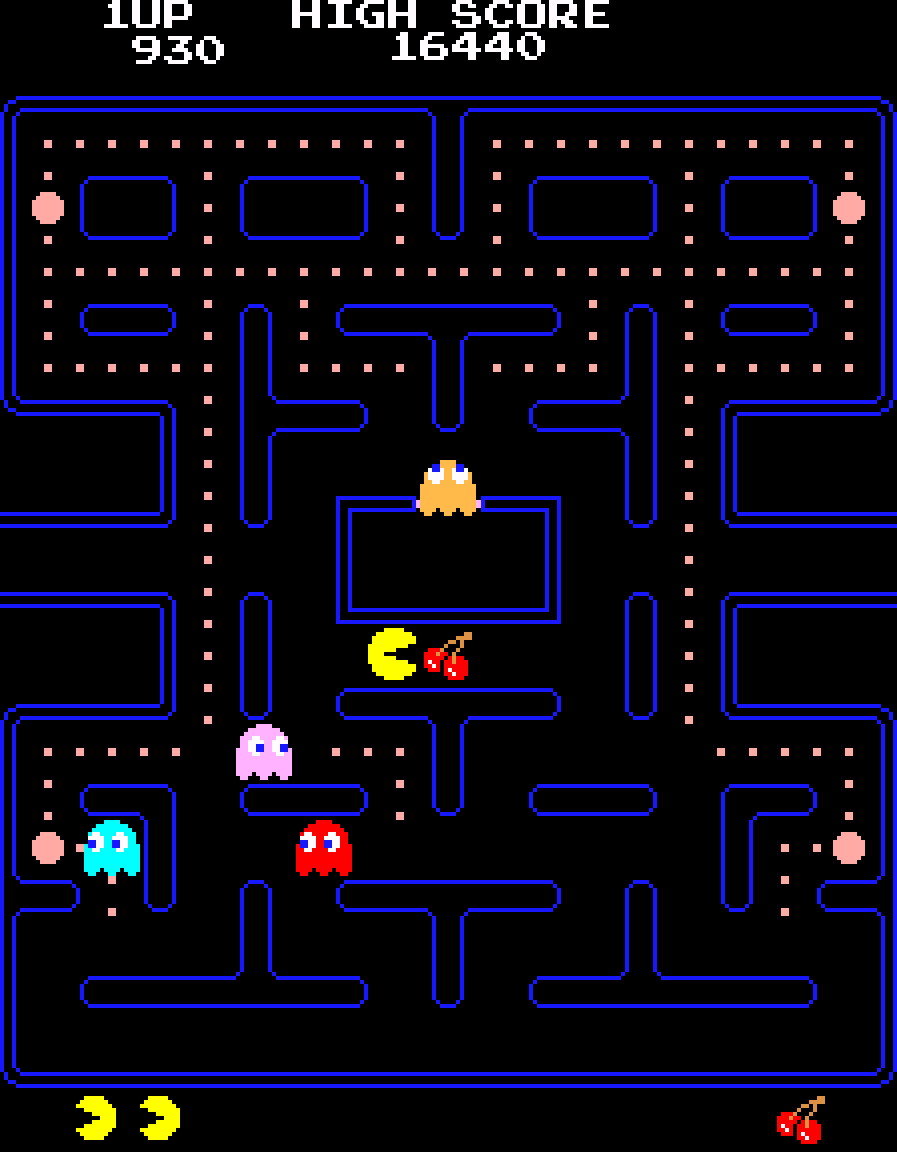
\includegraphics[scale=0.5]{files/pacman.jpg}
      \caption{Esquema del Juego\footnotemark{}.}
    \end{figure}
    \vspace{-1cm}
    \footnotetext{\bibentry{examplepacman}}
\end{frame}

\subsection{Aplicación de Inferencia Bayesiana}

\begin{frame}{MODELO Y APLICACIÓN}
    \framesubtitle{Aplicación de Inferencia Bayesiana}
    \begin{itemize}
        \item Juego original utiliza algoritmos de grafos para encontrar el camino más corto hasta el nodo en que está el jugador.
        \item El juego está representado por nodos y aristas, en los nodos, el jugador puede cambiar su dirección.
        \item Inferencia para predecir dónde estará el jugador y desplazarse hasta allí.
    \end{itemize}

    \textbf{Variables}
    \begin{table}[H]
    \centering

    \begin{tabular}{l p{8cm}}
    \hline
     $N_{t+k}$ & Este es el nodo en el que estará el jugador en un tiempo $t+k$. No se puede considerar en un tiempo $t+1$.\\
     $P_t$ &  Es un punto con coordenadas $(x,y)$ en donde está el PacMan en un instante $t$.\\
     $V_t$ &  Es un vector de velocidades $(velX,velY)$ del PacMan en un instante $t$. Sólo puede tomar 4 posibles valores.\\ \hline
    \end{tabular}
    \caption{Variables del modelo.}
    \end{table}
    \end{frame}

    \begin{frame}{MODELO Y APLICACIÓN}
        \framesubtitle{Aplicación de Inferencia Bayesiana}
        \begin{itemize}
            \item Comportamiento modelado a través de una Cadena de Markov.
            \item Los fantasmas comienzan moviéndose hacia un nodo aleatorio.
            \item No puede calcularse cada vez que el jugador se mueve, busca el nodo más probable y se mueve hacia allí. Se repite el proceso.
            \item Se debe calcular:
            \begin{equation}
                \small P({ N }_{ t+k }=n\mid { P }_{ t }=p\wedge { V }_{ t}=v)=\frac{P({ P }_{ t }=p\wedge { V }_{ t}=v\mid{ N }_{ t+k }=n)P({ N }_{ t+k }=n)}{P({ P }_{ t }=p\wedge { V }_{ t}=v)}
            \end{equation}
        \end{itemize}
    \end{frame}
